\section{Hoveddel} 2 til 4 situasjonsfortellinger Teori og begreper
flettes inn underveis Refleksjoner rundt situasjonene, både individ- og
gruppenivå Aksjoner (tiltak/videreføre, reflektere)

\subsection{Gruppens kommunikasjonsmønster} %gruppelogg 08.02 
Under en av gruppens diskusjoner 8. februar fikk vi en tilbakemelding av
fasilitator på hvordan kommunikasjonen i gruppen utartet seg. For å gå
inn i dybden på dette kan det nevnes hvordan stemningen på gruppen var
på starten av dagen. Forrige onsdag fikk vi utviklet en idè som alle på
gruppen var fornøyde med. Etter flere timers arbeid med dette hadde vi
en oppsummering sammen med landsbyens leder for å oppdatere henne på
hvordan vi lå an. Det viste seg at idèen vår ikke var bra nok med tanke
på at resirkulering ikke stod som hovedfokus. For å følge opp
problemsstillingen vår og landsbymålene måtte vi gjøre store endringer.
Dette ble en dårlig avslutning på dagen, og motivasjonen sank
betraktelig.

Da vi møtte opp onsdag 8. februar var den generelle stemningen på
gruppen at medlemmene var demotiverte. Det at idèen vår fra den
foregående onsdagen føltes som bortkastet lå fortsatt i tankene til alle
på gruppen. Kjetil nevnte at han var lite klar for å gå tilbake et
skritt og gå gjennom en helt ny idèmyldring, ettersom vi forrige gang
endelig følte at vi hadde en idè som alle var fornøyde med. Dette
utsagnet var ikke akkurat noe som bidro til en bedre start på dagen for
resten av gruppen. Trond og Andreas tenkte at man bare må gjøre det
beste utav det, og de startet en diskusjon som gikk ut på å dekomponere
idèen vår fra forrige gang. Kjetil kastet seg for på, og motivasjonen
hans økte når han innså at dette kanskje ikke var verdens undergang.
Etter en tid med brainstorming videreutviklet og endret vi det vi jobbet
med forrige onsdag. Lydnivået økte og motivasjonen på gruppen steg
blandt flere av medlemmene. En ny idè ble født.

Da Andreas følte at gruppen virkelig var i sving, kom fasilitator bort
til gruppen med en skisse som viste hvordan kommunikasjonen på gruppen
var.
\begin{figure}
\begin{center}
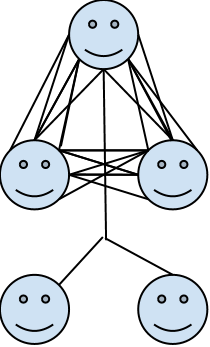
\includegraphics[scale=0.5]{communication}
\caption{Kommunikasjonsmønster}
\end{center}
\end{figure}
Dette kom som en overaskelse på gruppen. Det viste seg at Andreas,
Kjetil og Trond var mest aktive, mens Ina og Christian var mer passive.
Dette måtte diskuteres i gruppen.  Ina mener at årsaken til hennes
passivitet er i tråd med hennes vanlige oppførsel under et gruppearbeid.
Hun sier at hun er meget observant og enig i det som skjer, men at hun
ikke alltid legger merke til at hun kan virke passiv for resten av
gruppen. Når hun er enig tenker hun ikke over å si dette til resten av
gruppen, eller gi de andre hennes godskjennelse. Hvis hun derimot er
uenig sier hun ifra. Hun understreker at hun ikke er tilbakeholdende
eller ukomfortabel med å si ting foran hele gruppen. Ina sier at hun
føler seg like aktiv som de andre selv om hun snakker mye mindre. Dette
er derimot ikke resten av gruppens oppfatning, som i dette tilfelle
oppfattet henne som passiv. 

Kjetil mener at man henvender seg til de som er mest aktive, ettersom
man får mer respons fra dem. Andreas sier at grunnen til at vi ikke
inkluderer alle ikke har noe med at man trenger “godkjenning” fra
enkelte av gruppenes medlemmer, men at diskusjonen hoper seg opp der
folk er mest aktive. Dette observerte Andreas senere på dagen, da
mønsteret flyttet på seg. 

Christian var veldig trøtt på morgenen, og merket at han var litt i
kjelleren. Etter en kaffekopp ble han mer sentral i diskusjonen. Etter
at vi ble observante på hvordan dette mønsteret var, tok vi en pause;
for å tenke litt på andre ting, ta en kaffe, og reflektere litt over
hvorfor det var slik. 

Det var ingen tvil om at aktiviteten på gruppen ble mer balansert etter
denne pausen. Vi ble klar over hvem vi henvender oss til når vi snakker.
Andreas sa senere at han begynte å ta dette i betrakning i senere
diskusjoner, der han beveger blikket mer for å få visuell kontakt med
alle på gruppen. Trond foreslå at man kan legge til spørsmål til
gruppemedlemmene om de er enige eller uenige, og rette disse mot dem på
gruppen som er mer passive. Ifølge Schwarz \cite{Schwarz} er det å invitere til drøfting av egne innspill en god måte å øke effektiviteten i gruppen på. Dette bidrar til å få mer kommunikasjon
mellom alle på gruppen, og inkluderer dem som kan være umotiverte og
trøtte eller ikke kommuniserer like mye. 

Gruppen ble også bevisst på et annet problem under videre diskusjon om
spillidèen. Idèen utviklet seg raskt og det var stor enighet i gruppen.
Men da vi begynte å tegne og visualisere idèen viste det seg at flere av
gruppemedlemmene så for seg forskjellige ting. Selv om kommunikasjonen
så ut til å fungere etter situasjonen om gruppens kommunikasjonsmønster,
var det likevel store forskjeller i hva de forskjellige medlemmene
trodde vi diskuterte. Her har Schwarz en teori om at man ved å dele all relevant informasjon, spille med åpne kort og avdekke resonnementene bak de innspillene man kommer med vil hjelpe gruppen i å arbeide effektivt sammen. Ved å gå mer i dybden på det vi diskuterte, snakke om
detaljer og være klar over at folk tenker forskjellig førte videre til
at slike misforståelser ble unngått. Det å kartlegge slike ulikheter
kan også brukes som en fordel i gruppen. I neste avsnitt reflekteres det
over denne situasjonen i forhold til gruppemedlemmenes ulike tankegang.

%johnson, kap 10.
Johnson \& Johnson  \cite{Johnson} understreker viktigheten av mangfold
i en gruppe. I forhold til denne situasjonen er ulike personligheter et
viktig bidrag til en gruppe. Det at gruppens medlemmer tenker
forskjellig kan virke frusterende når man skaper en idé. Hvis gruppen
klarer å kartlegge disse ulikhetene kan gruppemedlemmenes ulike
tankegang bidra til å skape noe større og bredere enn hvis alle på
gruppen hadde hatt helt lik tankegang. Personlige karaktererforskjeller
på vår gruppe er kjønn, studieretning og ulike verdier og meninger. I
tillegg har vi ulike egenskaper og ulik kunnskap. De på gruppen som
studerer datateknikk er mer likesinnede og har ofte like forestillinger
under idèutviklingen. De tar hensyn til programmering og gjennomføring
av spillet, noe som Andreas og Ina ikke tenker på, ettersom de ikke har
noe kunnskap innen dette feltet. Men Ina og Andreas tar andre ting i
betrakning under idèutviklingen, der blandt annet inkorporering av
biologi og geologi i spillet står sentralt. Dette fører til at når vi i
den nevnte situasjonen kommer frem til noe alle er enige i, betyr ikke
dette at man vet hva man er enige om. Fordi gruppens medlemmer har ulike
bilder i tankene om hvordan de ser for seg denne idèen. Vi fant ut at
dette var tilfelle. Så hvordan kan vi dra nytte av dette?  I
utgangspunktet skulle man tro at en homogen gruppe som består av
datastudenter er det optimale i gjennomførelsen av et slikt prosjekt.
Johnson \& Johnson nevner flere ulemper ved en lik gruppe. I denne
situasjonen skal vi nevne en av disse ulempene. En slik gruppe kan
mangle et bredt perspektiv. Kjetil, Trond og Christian hadde
antageligvis klart å lage et kjempebra produkt, men med en homogen
tankegang er det antageligvis mange ting de ikke har tenkt over. Ina og
Andreas, som ikke har kunnskaper innen programmering, ser på oppgaven i
et annet perspektiv enn resten av gruppen. De har ikke noe å bidra med
rent teknisk til resultatet, men de ser på ting annerledes og kaster lys
over oppgaven på en måte datastudentene ikke tar i betrakning. Da vi
prøvde å flette sammen hver persons synspunkt på hva vi trodde vi hadde
kommet frem til, førte dette til at hele gruppen endret sin personlige
idè over hva vi hadde diskutert og gjorde det om til gruppen sin idè.
Dette resulterte i noe ingen på gruppen hadde sett for seg, men som alle
var veldig fornøyde med.  Kjetil mente først at denne diskusjonen var
sløsing og tid og så på dette som en unødvendig del av gruppearbeidet.
Men den idèen gruppen satt igjen med på slutten av dagen fikk Kjetil til
å tenke annerledes. Han ble overrasket over at hans eget syn på
dataspillet vi utviklet ble såpass endret da de andre på gruppen
fortalte hva de tenkte. 

Ulike synspunkt og meninger, i tillegg til ulik faglig kompetanse og
tankegang, førte til et resultat ingen på gruppen så for seg i starten,
men som alle var meget fornøyde med. Vi klarte å dra nytte av disse
ulikhetene.
